In \Chapter{ch:speckle} the statistics of cone speckle, the intensity PDF and
contrast, were shown to be in agreement with the random phasor sum model
(\Equation{eqn:phasorsum}).  Unfortunately, this model only serves to describe
the observation; it does not describe the underlying process.

Physically, there are two possible scattering processes which can occur
(\Figure{fig:scattsinglevmultiple}).  The first is \textit{single scattering},
whereby only one scattering event occurs in each path from source to
observation.  Since scattering is a general phenomena, paths may be traversed
by any phase recording object: a photon, SPP, electron, etc.; at the moment
the object is not important.  In addition to single scattering, there exists a
much more interesting and phenomenologically complex process known as
\textit{multiple scattering}.  In multiple scattering, each path from source
to observation contains multiple scattering events.  Both single
and multiple scattering produce speckle with identical first order statistics
as described by the random phasor sum model, and are difficult to distinguish
in this way.
\begin{figure}[ht]
\centering
\begin{subfigure}[b]{5cm}
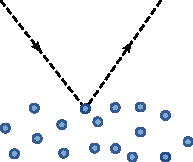
\includegraphics[keepaspectratio,height=4cm]{scatteringmicro/figures/singlescattering}
\caption{single scattering}
\end{subfigure}
\hspace{2cm}
\begin{subfigure}[b]{5cm}

\includegraphics[keepaspectratio,height=4cm]{scatteringmicro/figures/multiplescattering}
\caption{multiple scattering}
\end{subfigure}
\caption{Conceptual differences between single and multiple scattering.  In
single scattering, a path visits only one scatterer.  In multiple scattering,
many scatterers may be visited.}
\label{fig:scattsinglevmultiple}
\end{figure}

The transition from the single to the multiple scattering occurs roughly upon
fulfillment of the Ioffe-Regel criterion~\cite{ioffe1960non}, when the
transport mean free path $l^*$ is much larger than the spatial frequency of
the optical wave, or
\begin{equation}
k l^* \approx 1
\end{equation}
where $k=\omega/c$ as usual.  The transport mean path is defined as the
characteristic distance over which the incident wave is scattered out of
its incoming direction~\cite{berkovits1994correlations}.  This is the
optical analog of electron transport in condensed matter physics.  There,
one would use the Fermi wavenumber $k_F$ and take $l^*$ to be the mean free
path.  Materials for which $k_F l^* \gg 1$ are conductors, and materials
for which $k_F l^* \ll 1$ are insulators.  The multiple scattering regime can
also be defined in terms of the sample length $L$, such that if
$l^* \ll L$ and $1/(k l^*) \ll 1$, the system can be thought to be the
multiple scattering regime.  

\subsection{Correlations}
Though speckle from a single and multiple scattering process share the same
first order statistics (\Chapter{ch:speckle}), significant differences emerge
in correlations between speckle patterns when the system is perturbed.  

Consider the case of SPP single scattering from a collection of $N$
``scatterers'', i.e.\ defects on the two dimensional metal surface which
scatter SPPs out of plane into the cone.  The scatterers are given Cartesian
coordinates $(x,y,z=0)$, where the central point of the prism's hypotenuse on
the far surface of the metal film is the origin $(0,0,0)$.  The detector (a
two dimensional image sensor) has coordinates $(x^\prime,y^\prime,z^\prime)$.
The metal film is in the $x$-$y$ plane and the incident light in the $x$-$z$
plane.

The field on the detector has two phase contributions. The first,
$\varphi_\mathrm{loc}$, comes from
the phase of the local SPP field propagating on the metal surface in the $x$
direction,
\begin{equation}
\varphi_\mathrm{loc} = \ksp x.
\end{equation}
The second, $\varphi_\mathrm{ff}$, is phase accumulated from the scatterer into the far field,
\begin{equation}
				\varphi_\mathrm{ff} =
				k_0\sqrt{{(x-x^\prime)}^2+{(y-y^\prime)}^2+{(z-z^\prime)}^2}.
\end{equation}
Together, the field on the detector from a single scatterer is
\begin{align}
\mathbf{E}(x^\prime,y^\prime,z^\prime) &=
\mathbf{E}_0\exp\bigl(\mi(\varphi_\mathrm{loc}+\varphi_\mathrm{ff})\bigr)\\
&= \mathbf{E}_0\exp\!\left(\mi\ksp x + %
\mi k_0\sqrt{{(x-x^\prime)}^2+{(y-y^\prime)}^2+{(z-z^\prime)}^2}\right).
\end{align}
Or, in spherical coordinates with the detector at
$(\rho^\prime,\theta^\prime,\phi^\prime)$,
\begin{align}
				\mathbf{E}(\rho^\prime,\theta^\prime,\phi^\prime) &= \mathbf{E}_0\exp\Bigl(\mi\ksp x \\
&+ \mi k_0\sqrt{{(\rho^\prime\sin\theta^\prime\cos\phi^\prime
x+x)}^2+{(\rho^\prime\sin\theta^\prime\sin\phi^\prime+y)}^2+{(\rho^\prime\cos\theta^\prime+z)}^2
} \Bigr).
\label{eqn:scattspherical}
\end{align}
Note that the refractive index change from prism to air has been neglected.
To a good approximation, the hemispherical geometry imparts only a constant
phase to the sum, and therefore has no observable effect on the speckle
pattern.

For a collection of $N$ scatterers, a single scattering process produces $N$
unique phasors over $N$ paths where the $n$th path has 
phase $\varphi_n = \varphi_\mathrm{n,loc}+\varphi_\mathrm{n,ff}$.  In this
case, the field on the detector
is given by the superposition 
\begin{equation}
\mathbf{E}(x^\prime,y^\prime,z^\prime) =
\sum_{n=0}^{N-1}
\mathbf{E}_n \me^{\mi{(\varphi_\mathrm{n,loc}+\varphi_\mathrm{n,ff})}}
\end{equation}
where
\begin{equation}
\sum_{n=0}^{N-1}\mathbf{E}_n = \mathbf{E}_0.
\end{equation}

In the case of multiple scattering, another phase term,
$\varphi_\mathrm{ms,n}$, is included for each scattering path.
$\varphi_\mathrm{ms,n}$ accounts for the path visiting $K$ scattering sites with
positions $(x_k,y_k,z=0)$ on the two dimensional metal surface
\begin{equation}
\varphi_\mathrm{ms,n}=\sum_{k=0}^{K-2} \sqrt{{(x_{k+1}-x_k)}^2+{(y_{k+1}-y_k)}^2}
\end{equation}
The $K$ scattering sites are chosen amongst the $N$ total scatterers and may
include multiple visits to any given scatterer.  The field on the detector for
multiple scattering is then
\begin{equation}
\mathbf{E}(x^\prime,y^\prime,z^\prime) =
\sum_{n=0}^{N-1}
\mathbf{E}_n
\me^{\mi{(\varphi_\mathrm{n,loc}+\varphi_\mathrm{n,ff}+\varphi_\mathrm{n,ms})}}.
\end{equation}



If the detector is in the far field, $\rho^\prime\gg\lambda_0$,
\Equation{eqn:scattspherical} can be simplified.  First the additional optical
path length accumulated propagating through the prism is neglected.  Second,
if the path length \textit{difference} between the origin and the far field is
used, \Equation{eqn:dingusthusly} becomes
\begin{equation}
\mathbf{E}(\rho^\prime\gg\lambda,\theta^\prime,\phi^\prime) = \exp\!\big( \mi \ksp x
 + \mi k_0 \sin\theta^\prime \left(x\cos\phi^\prime+y\sin\phi^\prime\right)
 + \varphi\big)
	\label{eqn:primarystripes}
\end{equation}
where we have included the variable $\varphi$ to represent the complex phase term
from non-tip-scattering events (a coherent background).  



Such
correlations are amazingly difficult to compute analytically, and have up to
now only been determined for a limited number of systems with simple
transmission and reflection geometries~\cite{berkovits1994correlations}.
Furthermore, the mathematical methods used in such computations (Feynman
diagrams, ladder propagators, vertex operators, etc.) are beyond the scope of
this work.  

